\documentclass[letterpaper]{article}

\usepackage[margin=1in]{geometry}    % For margin alignment
\usepackage{algorithm}
\usepackage{algpseudocode}
\usepackage{amsmath}

\usepackage{graphicx}

\title{Resampling Algorithm Proposal}
\author{Mitchell Gilmore}

\begin{document}

	\maketitle

	\section*{Abstract}

	The purpose of this proposal is to suggest a resampling scheme that can be implemented to translate
	an arbitrarily sized finite signal from one sampling rate to another. Though the implementation
	is for a finite signal it will be written in such a way for easy translation for to use in a real
	time application. \newline

	\noindent
	This implementation will only implement a structure covered in class and will place the burden of an
	anti-aliasing filter design to the end user. For testing the filter for this application will be
	determined using prior software to determine an optimal filter. Future work may implement optimal
	filter selection, but it falls outside the scope of this proposal.

	\section*{Diagram}


	\begin{figure}[!ht]
		\centering
		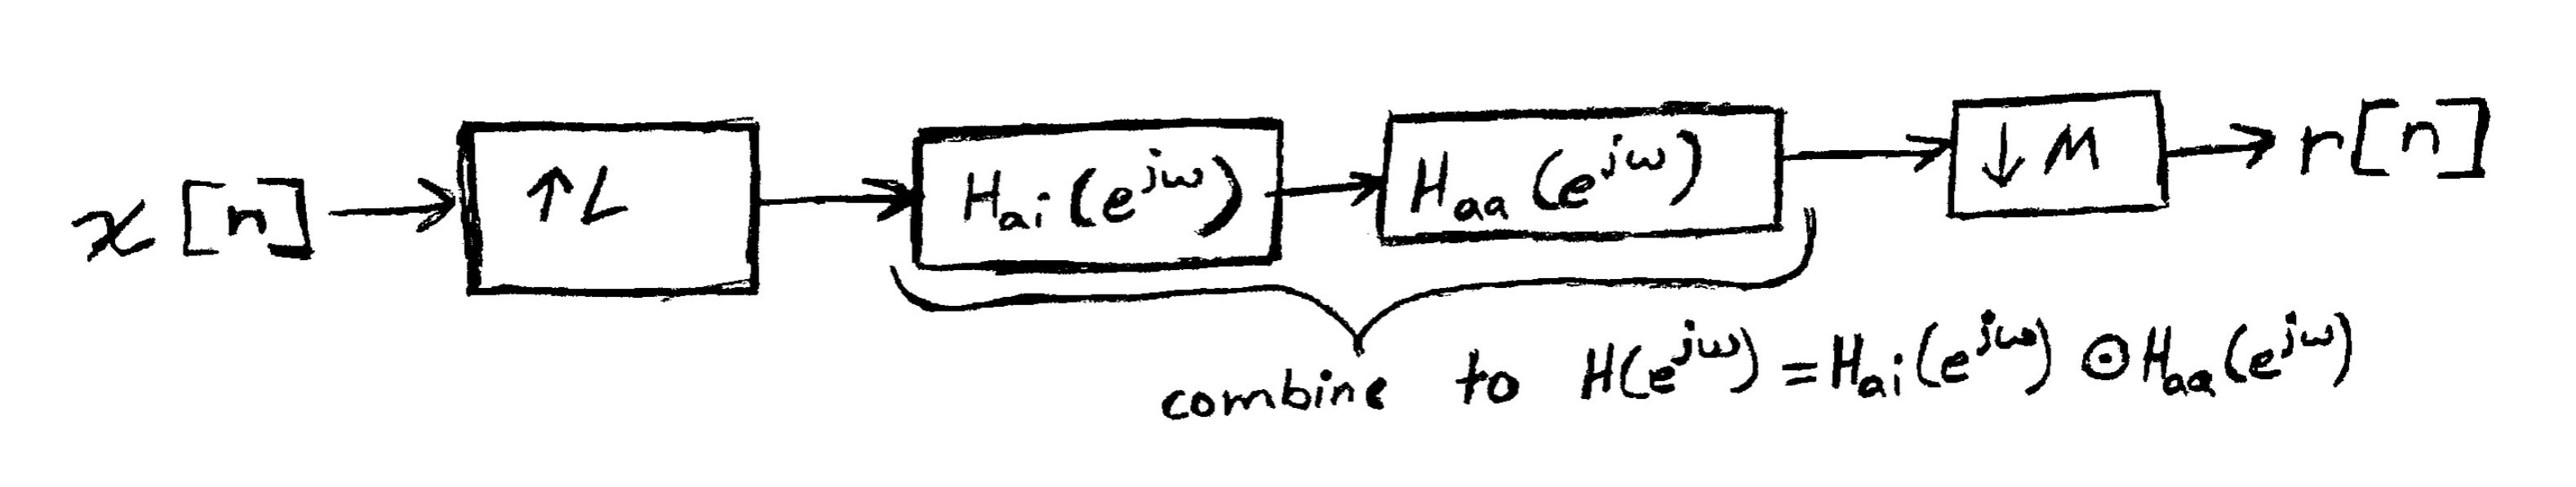
\includegraphics[scale=0.2]{figs/main.png}
	\end{figure}

	\begin{figure}[H]
		\centering
		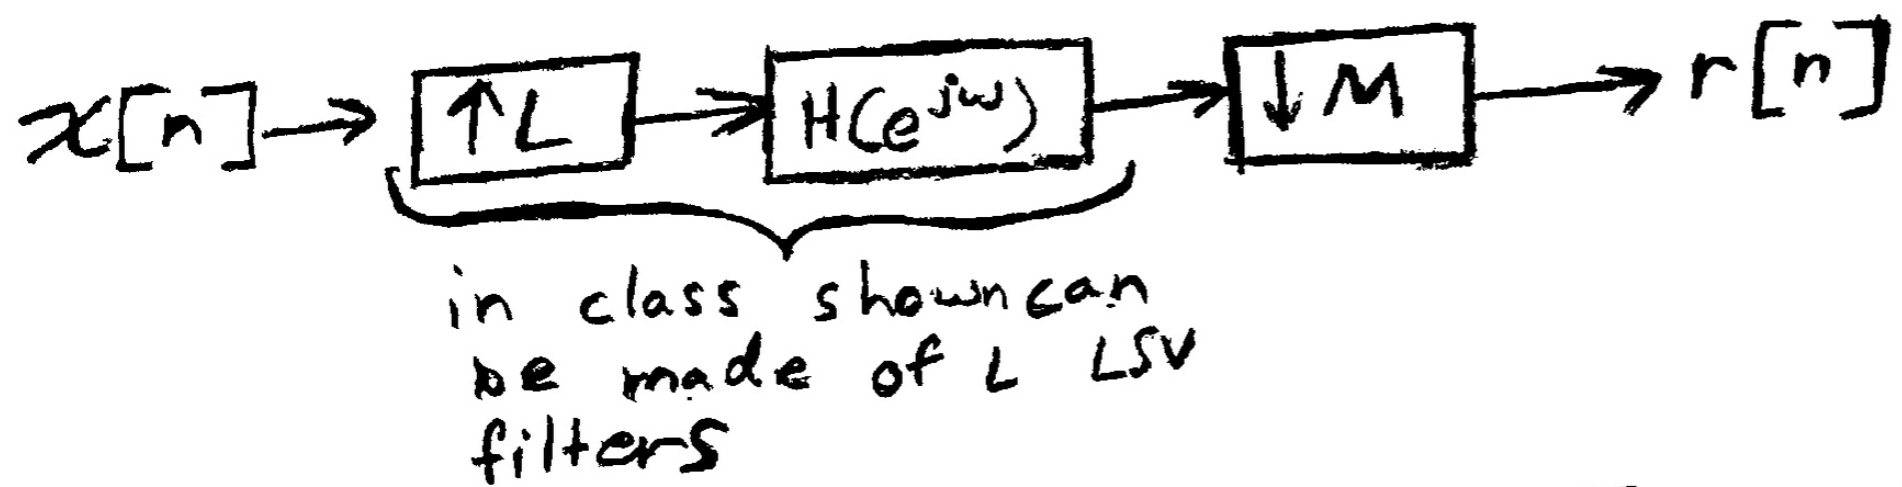
\includegraphics[scale=0.2]{figs/main2.png}
	\end{figure}

	\begin{figure}[H]
		\centering
		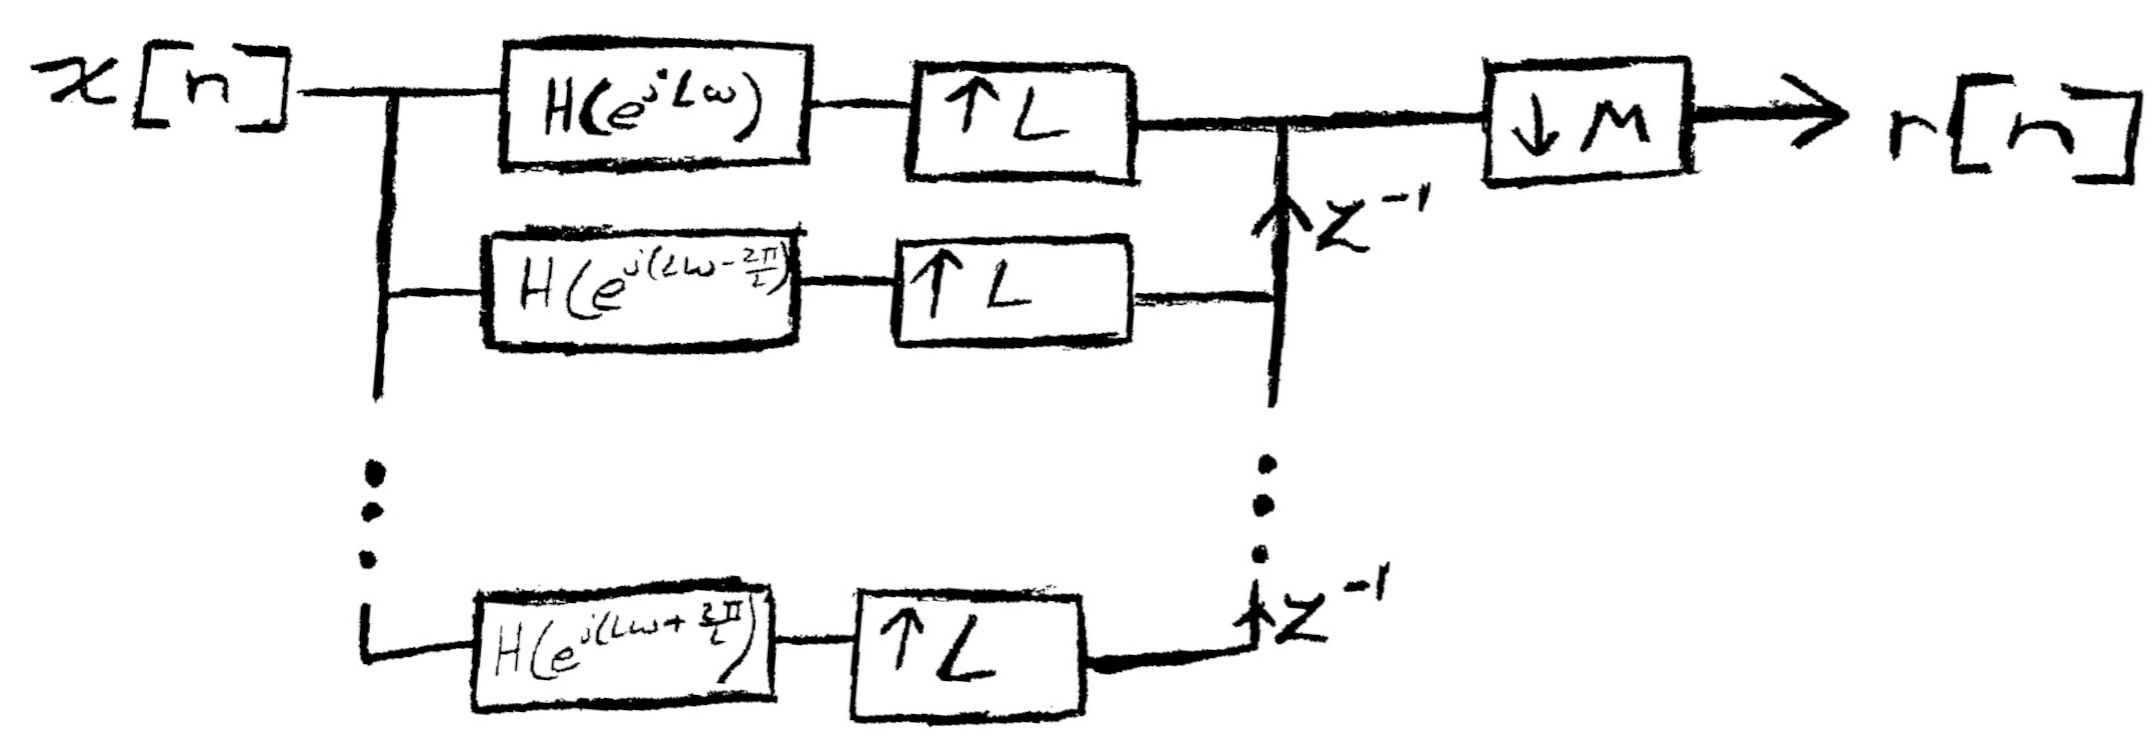
\includegraphics[scale=0.2]{figs/main3.png}
	\end{figure}

	\section*{Algorithms}

	\begin{algorithm}
		\caption{Resampler Initialization}
		\begin{algorithmic}[1]

		\Procedure{Resampler}{$f_{origin},f_{target}, H_{aa}$}

			\State $L \gets f_{target}$ \Comment{Initializes the resampling factors L and M}
			\State $M \gets f_{origin}$

			\While{GCF$(L,M) > 1$}             \Comment{loops through $L$ and $M$ until $L/M$ is optimal}
				\State $Z \gets$ GCF$(L,M)$ \Comment{Determines The Greatest Common Factor}
				\State $L \gets L / Z$    \Comment{Reduces $L$ and $M$ by a factor of Z}
				\State $M \gets M / Z$
			\EndWhile

			\State $self.L \gets L$ \Comment{Stores optimal $L$ and $M$ to object}
			\State $self.M \gets M$

			\For {$i$ in range$(L)$} \Comment{Partitions $H_{aa}$ into $L$ LSV filters}
				\State $self.h[i] \gets \text{reverse} (H_{aa}[i::M])$
			\EndFor

			\State \textbf{return} $self$

		\EndProcedure

		\end{algorithmic}
	\end{algorithm}

	\begin{algorithm}
		\caption{Resampler call}
		\begin{algorithmic}[1]

		\Procedure{Resampler.call}{$x$}

			\State $h_i  \gets 0$ \Comment{Initializes filter index}
			\State $o_i  \gets 0$ \Comment{Initializes origin array index}
			\State $t_i  \gets 0$ \Comment{Initializes target array index}
			\State $h_l \gets$ len$(self.h[h_i])$ \Comment{gets current LSV filter length}

			\While{$o_{i} + h_{l} <$ len$(x)$} \Comment{loops until out of data}
				\State $t[t_i] \gets \langle x[o_i: o_i + h_l], self.h[h_i] \rangle$ \Comment{inner product between $x$ and $h$}
				\State $t_i \gets t_i + 1$ \Comment{sets data for next iteration}
				\State $h_i \gets (h_i + self.M) \mod self.L$
				\State $h_l \gets$ len$(self.h[h_i])$
				\State $o_i \gets o_i + \lfloor (h_i + self.M) / self.L \rfloor$
			\EndWhile

			\State \textbf{return} $t$

		\EndProcedure

		\end{algorithmic}
	\end{algorithm}


\end{document}